\documentclass{memoir}
\usepackage[spanish]{babel}
\usepackage[utf8]{inputenc}
\usepackage{graphicx}

\pagestyle{empty}

\begin{document}
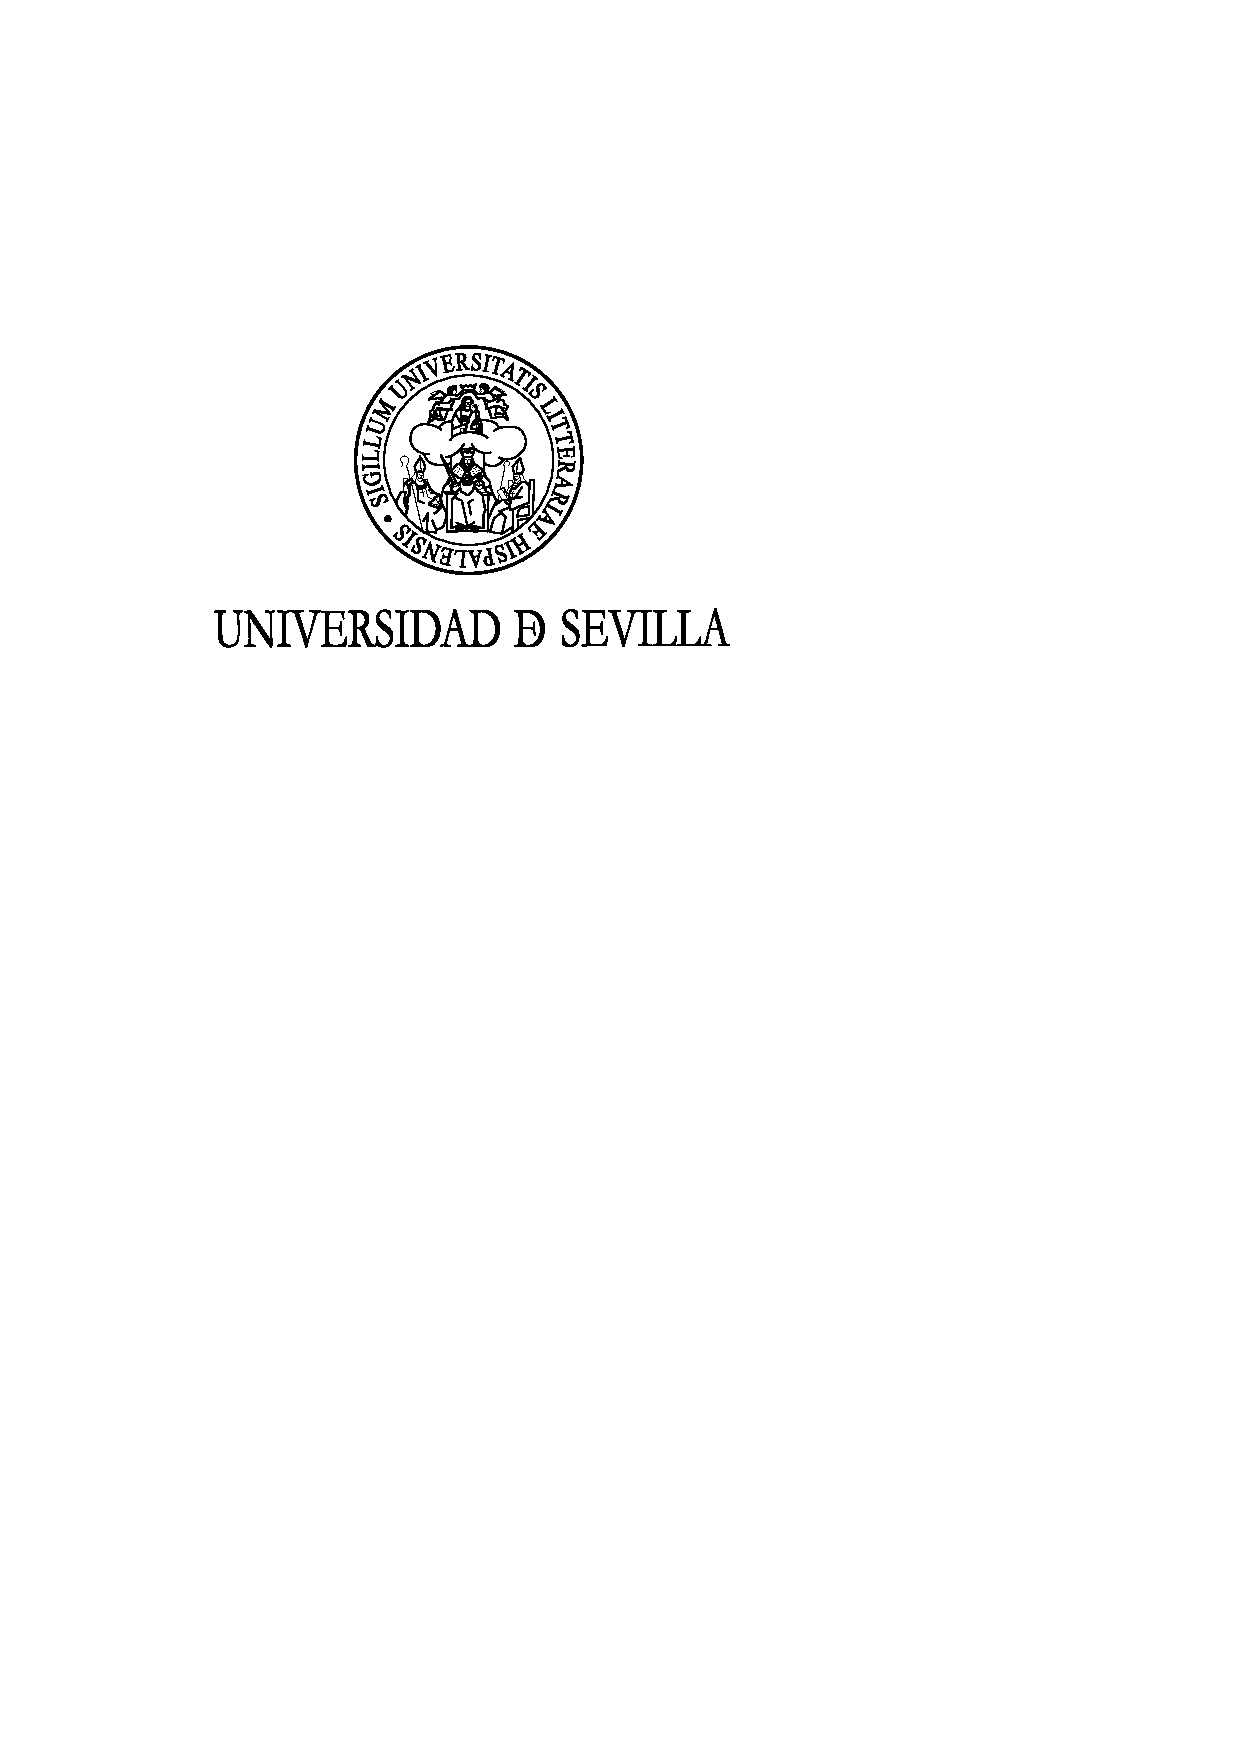
\includegraphics[scale=.5]{ /Users/fernandomurojimenez/Documents/comisiondeservicios/.venv/lib/python3.12/site-packages/csus/logo.pdf}
\begin{vplace}[.5]
\vspace{1cm}
\textbf{Fernando Muro Jiménez}, miembro del proyecto MTM-3000-4000.

\vspace{1cm}

\textbf{QUIERO HACER CONSTAR QUE:}

\vspace{1cm}

Entre los días 6 y 10 de junio de 2022, viajé a Boston, Massachusetts, USA, para asistir al congreso "Mathematical models with industry patterns", organizado por el Massachusetts Institute of Technology. Este evento fue una gran oportunidad para investigar aplicaciones de la algebra en la criptografía (O2) y explorar su uso en algoritmos de aprendizaje automático (O5). Además, el congreso propició la colaboración con socios de la industria, lo cual es fundamental para aplicar la investigación matemática en contextos prácticos (O8).

Durante mi participación, también me enfoqué en mejorar métodos computacionales para resolver ecuaciones algebraicas (O3), analizando cómo la matemática juega un papel crucial en la seguridad de redes (O6). La discusión sobre nuevos modelos matemáticos para sistemas complejos (O1) fue especialmente relevante, ya que estos modelos tienen un impacto significativo en la ciencia de datos (O4). Por último, este tipo de congresos fomenta la publicación de hallazgos en revistas científicas de alto impacto (O9) y la organización de talleres y conferencias para difundir la investigación (O10), contribuyendo así al desarrollo de herramientas educativas para la enseñanza del álgebra avanzada (O7). 

\vspace{1cm}

Y para que conste a los efectos oportunos, firmo el presente escrito en Sevilla, a \today.

\vspace{3cm}

\begin{flushright}
    Fdo.: Fernando Muro Jiménez 
\end{flushright}
\end{vplace}
\end{document}